\graphicspath{{figures/}}
% Header
\renewcommand\evenpagerightmark{{\scshape\small Introduction}}
\renewcommand\oddpageleftmark{{\scshape\small Chapter 1}}

%\renewcommand{\bibname}{References}

\hyphenation{}

\chapter[Introduction]%
{Introduction}
\label{ch1}

\begin{flushright}
\begin{quotation}
In order for the wheel to turn, for life to be lived, impurities are needed, and the impurities of impurities in the soil, too, as is known, if it is to be fertile. -- Primo Levi --
\end{quotation}
\end{flushright}
\npar

Catalysis, from the greek for ``down'' and ``loosen'', is at the heart of almost every industrially relevant chemical process. A catalyst intervenes in the reaction mechanism, allowing chemical species to meet each other and react with a specific mechanism, without being consumed. Not only can it increase the rate of a given reaction, allowing processes that would not happen spontaneously, but it can also steer the reaction to specific end products, allowing selectivity. Catalysts can be divided in homogeneous and heterogeneous, according to the phase where they are located with respect to the reactants. Homogeneous catalysts share the same phase with the reactants, and can be for instance molecules dissolved in a solvent, such as with organometallic compounds. These type of catalysts are used in many industrial processes,  but have the drawback of being difficult to separate from the products. From a modeling and experimental point of view, they are the easiest to study, and it is easier to hypotesize reaction mechanisms from experimental data. Heterogeneous catalysts, on the other hand, are located in a different phase with respect to the reactants, and for this reason they have the advantage of being easily separable from the reaction products. Even if the term does not refer to a specific phase, often heterogeneous catalysts is synonymous for solid catalysts. In order to exert their function, these materials must possess specific active sites that are easy to reach for the reactants, where these can adsorb, react, desorb, and ultimately diffuse back in the bulk to leave space for a new cycle. For these processes to occur, the number of active sites and the area of contact between the two phases (or surface area) must be sufficiently high. In this sense, nanoporous materials, which possess pores with diameter of <100 nm, have drawn a lot of attention for their enormous catalytic potential. Their pore structure provides them with an exceptionally high surface area, facilitating diffusion of reactants inside the material, and allowing shape selectivity to give specific products. In general, the study of solid heterogeneous catalysts is more difficult than their homogeneous counterparts due to their higher complexity. It is not always clear, in fact, where exactly the active sites may be located in the material, and how they interact with molecules. Moreover, these materials are far from perfect, and it is often the imperfections they contain that give them their catalytic properties. In this sense, computational design offers a perfect platform not only to understand the behavior of heterogeneous catalysts, but also to understand structure-activity relationship and design structures to target specific applications. Example of industrally relevant nanoporous heterogeneous catalysts are zeolites, which have been the workhorses of petrochemistry for the last decades. In this work of thesis, we focus on a new class of nanoporous materials which combine the crystalline nanoporous structure of zeolites with the versatility in synthesis of metal complexes and for this reason has shown great potential for catalysis.

\begin{figure}[!htbp]
	\centering
 	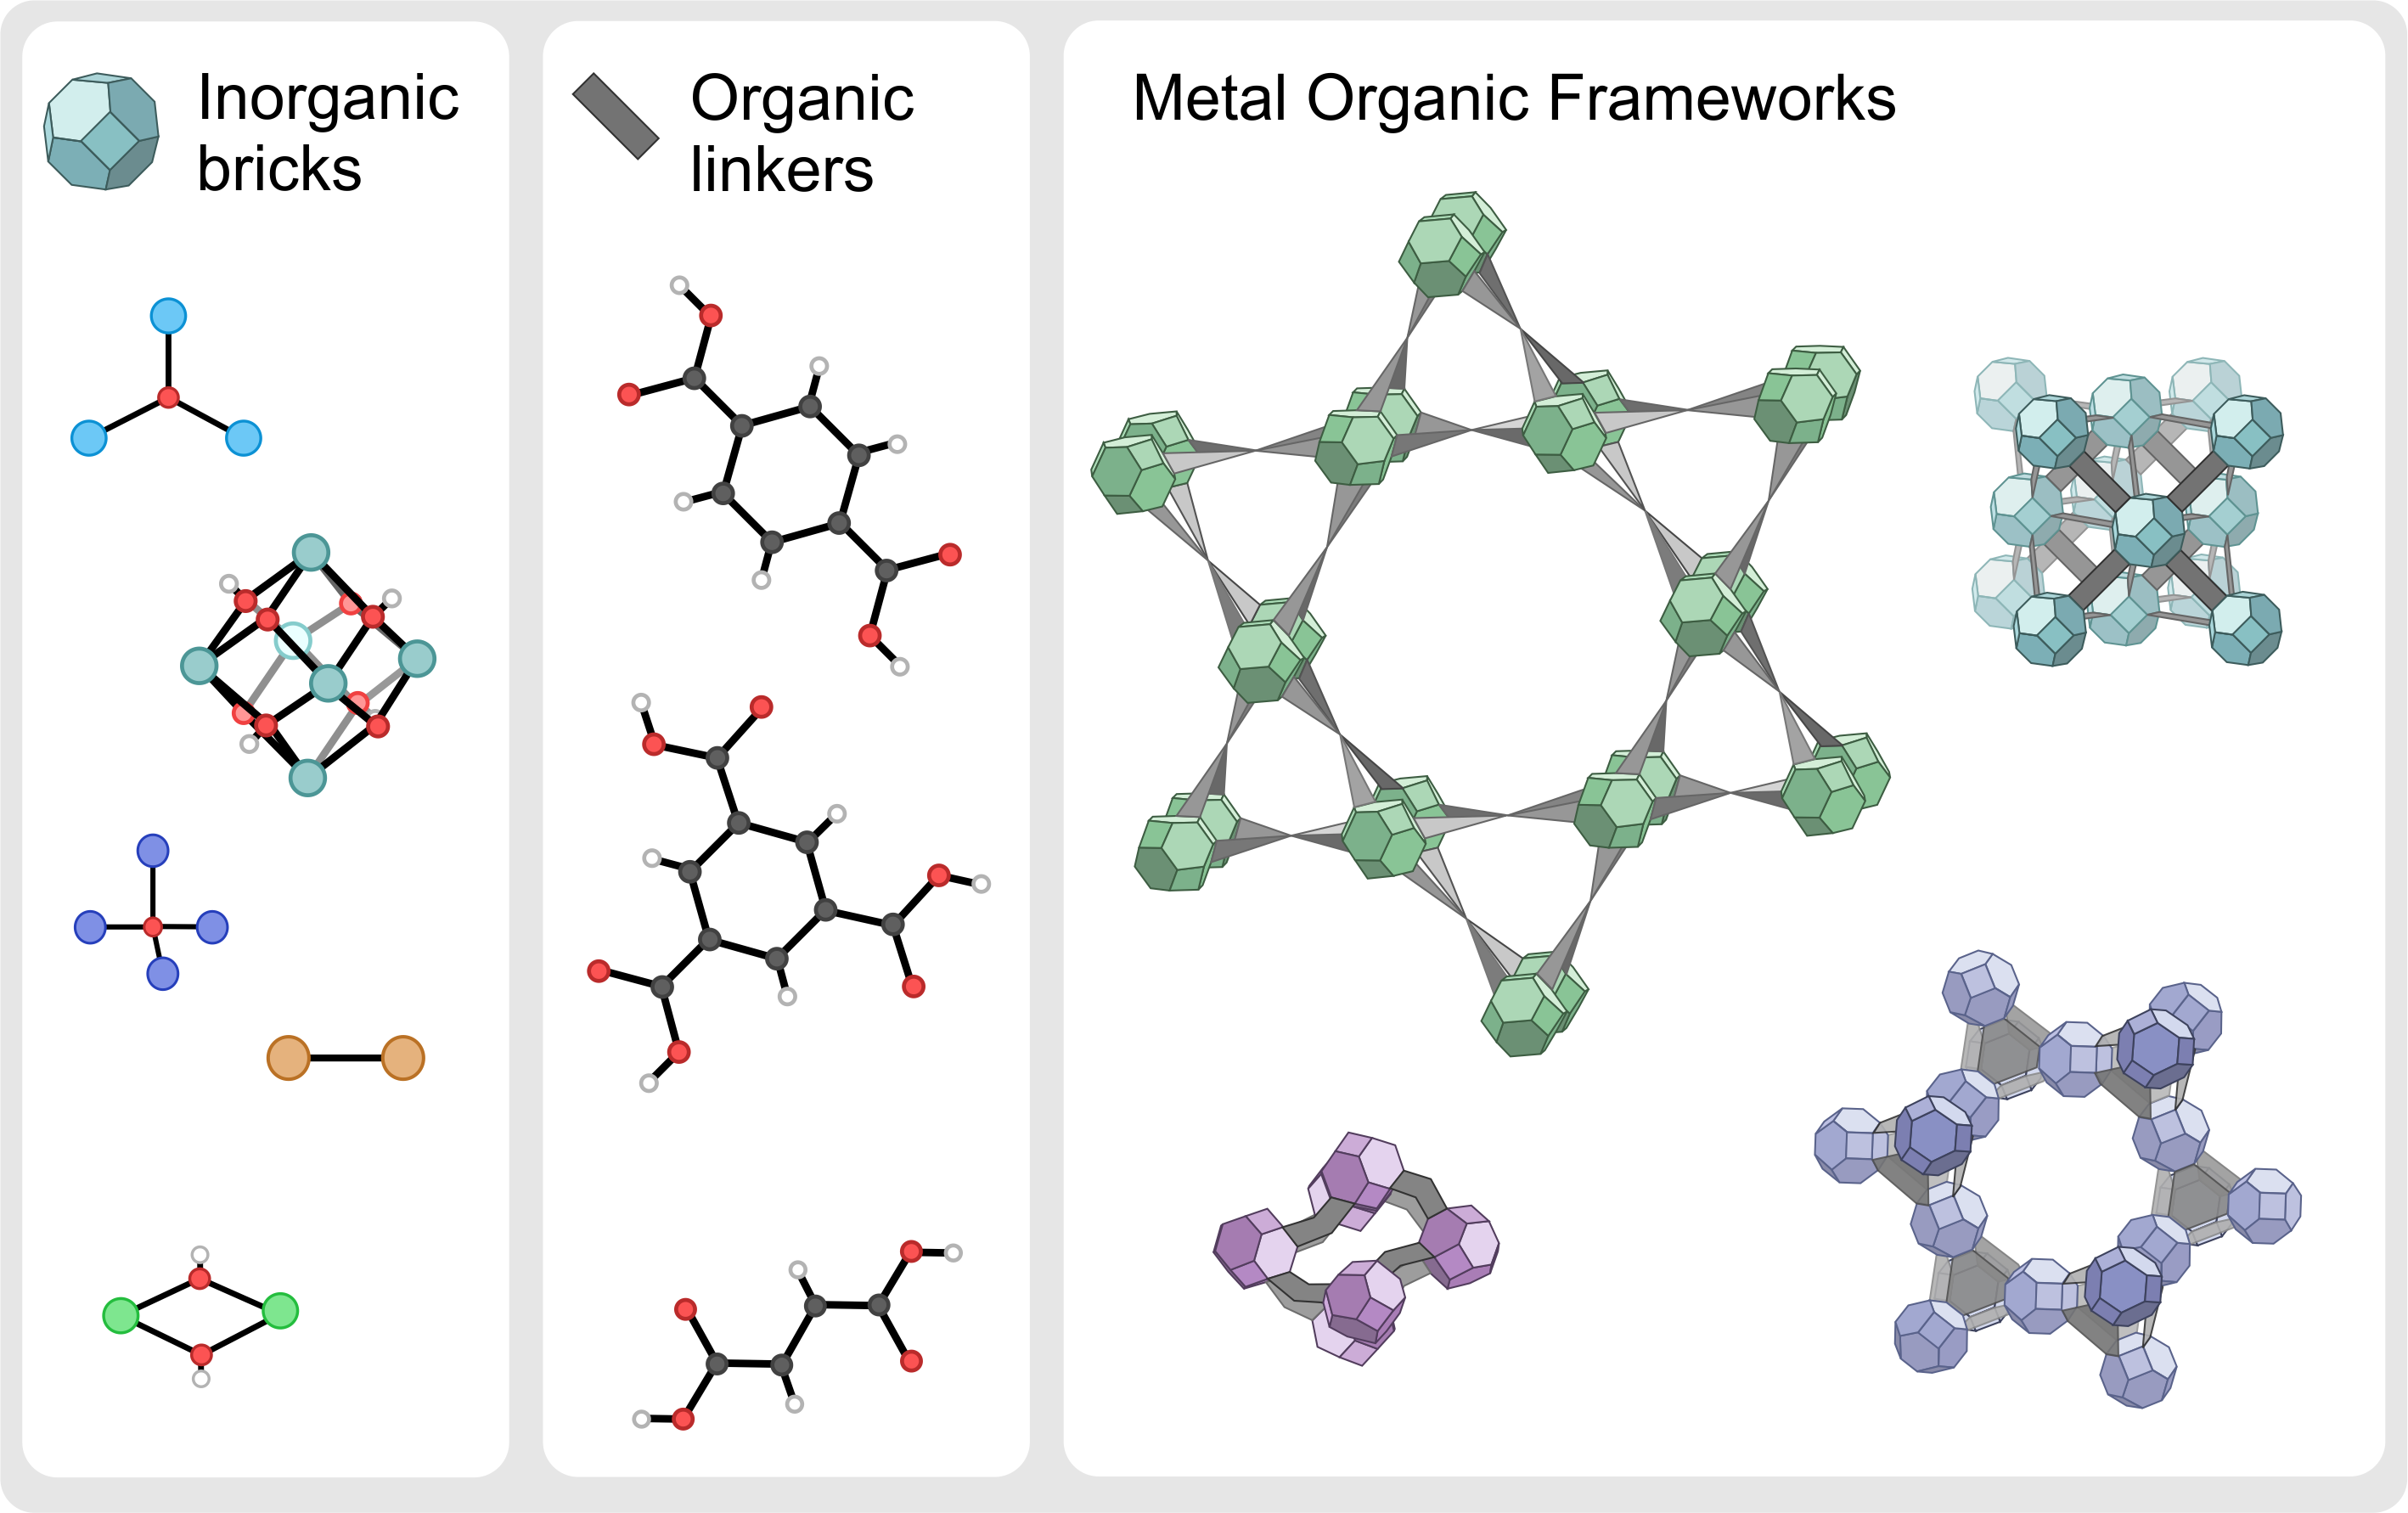
\includegraphics[width=1.0\textwidth]{MOFs}
	\caption{Schematic representation of the building block design in Metal-Organic Frameworks}
	\label{fig:MOFs}
\end{figure}

\section{Metal Organic Frameworks}
Metal organic frameworks (MOFs) are one of the most intriguing class of materials of current science. These promising materials, first called 'porous coordination polymers' (PCPs) were discovered in the late 50's, but only at the end of the century with the works of Robson\cite{batten1995two,hoskins1990design}, Kitagawa\cite{kitagawa1991synthesis, kitagawa1993synthesis}, Yaghi\cite{yaghi1995hydrothermal} and Ferey\cite{riou1998hybrid}, the scientific community started to understand their full potential. If at first these materials were seen as a laboratory curiosity, with the focus on the discovery of new structures, in the last few decades, the field has seen an incredible explosion in scientific and industrial interest, with new applications being continuously explored\cite{furukawa2013chemistry}. MOFs are hybrid nanoporous materials that are composed by metal or metal--oxo clusters connected by multitopic organic linkers, to form multidimensional pore structures. Compared to the already established zeolites, MOFs can be constructed without templating agents, with a far greater number of metals and with an exceptional structural diversity. In fact, their particular building block design (Fig. \ref{fig:MOFs}), that makes use of secondary building units (SBUs), allows the creation of an almost infinite number of crystalline structures with different topology and chemical composition. In principle, the nature of the SBUs and their association can be finely tuned\cite{stock2011synthesis}, allowing control on properties such as pore shape and size, functionalization, surface area, or response to chemical and physical stimuli\cite{zhou2014metal,zhou2012introduction}. Moreover, multiple physical or chemical functionalities can be integrated in the crystals at the same time\cite{li2016applications}. 
This tunability, along with their high cristallinity, metal content and porosity, allows their application in different industrially relevant fields, such as catalysis, gas storage and separation, drug delivery or sensing. More specific applications are being further explored, such as warfare agents decomposition, magnetic applications, or membrane separation. 
After the discovery of MOFs, with their tunability and ease in functionalization, the study of their application in catalysis followed naturally, and was one of the earliest documented applications\cite{Fujita1994}. 
%%
\begin{figure}[htbp]
	\centering
 	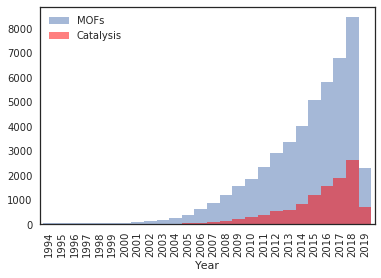
\includegraphics[width=1.0\textwidth]{citation_report}
	\caption{Number of publications on MOFs and catalysis in MOFs in the past 25 years (source: WebofScience)}
	\label{fig:citation_report}
\end{figure}
%%
Their high porosity, in particular, allows chemical species to diffuse in the pores and access the active sites, and the high metal content offers the possibility to have many guest interactions sites. Exploiting this property, a plethora of MOFs has been synthesized possessing unsaturated metal sites within the pores which offer different Lewis acidity. In this sense, provided the structures are stable at reaction conditions (i.e. no leaking is observed), MOFs can be considered true heterogeneous catalysts, where the active sites are inherent part of the framework. 
We can differentiate between three generations of porous systems, following the nomenclature proposed by Kitagawa\cite{kitagawa1998functional}. First generation MOFs are defined as having a guest--molecules supported pore system that collapses when these are evacuated, and for this reason found very limited use for practical applications. Those of second generation are more robust and have permanent porosity that is retained even in absence of guest molecules. These materials show high potential for catalysis and other applications and are the main object of this dissertation. Finally, third generation MOFs are characterized by flexible pores that can reversibly change shape with the presence of guest molecules, or upon certain stimuli, such as temperature or pressure. 
\begin{figure}[htbp]
	\centering
 	\includegraphics[width=1.0\textwidth]{mof-applications}
	\caption{Some of the applications of MOFs}
	\label{fig:mof-applications}
\end{figure}

\subsection*{Post--synthetic modification}
One of the most intriguing concepts is the isoreticular synthesis, by which inorganic or organic SBUs can be replaced by topologically identical (or similar) building blocks, giving rise to whole MOF families which derive from a specific precursor and span a range of pore size and functionality. For instance, the pore size can be significantly increased up to the mesoporous range by using longer isoreticular linkers, such as in the IRMOF series\cite{eddaoudi2002systematic}. When it is not possible to introduce functionalities with direct synthesis, post synthetic modification\cite{wang2009postsynthetic}, which makes use of the building block design, has become a well established procedure that allows the preparation of MOF materials with specific functionality. Via this technique, it is possible to modify the crystal after the synthesis, allowing to finely tune the properties of the material. Post synthetic modifications include encapsulation of guest molecules or nanoparticles in the pores, modifications of the linkers without breaking the metal--ligand bond, or post synthetic exchange (PSE) of linkers and metals, where building blocks are dynamically exchanged. 
PSE can also involve terminal ligands, or ligands adsorbed on the bricks that do not function as linkers, such as modulators. This way, building blocks can be exchanged, but also eliminated to create vacancies if the stability of the material allows it. Defect--containing MOFs have become an active field in MOF research, as defect sites can play a key role in the performance of the material. Post synthetic modification has been used as a strategy to efficiently introduce defective sites in MOFs. 

\subsection*{Zr--based MOFs}
%%
\begin{figure}[!htbp]
	\centering
 	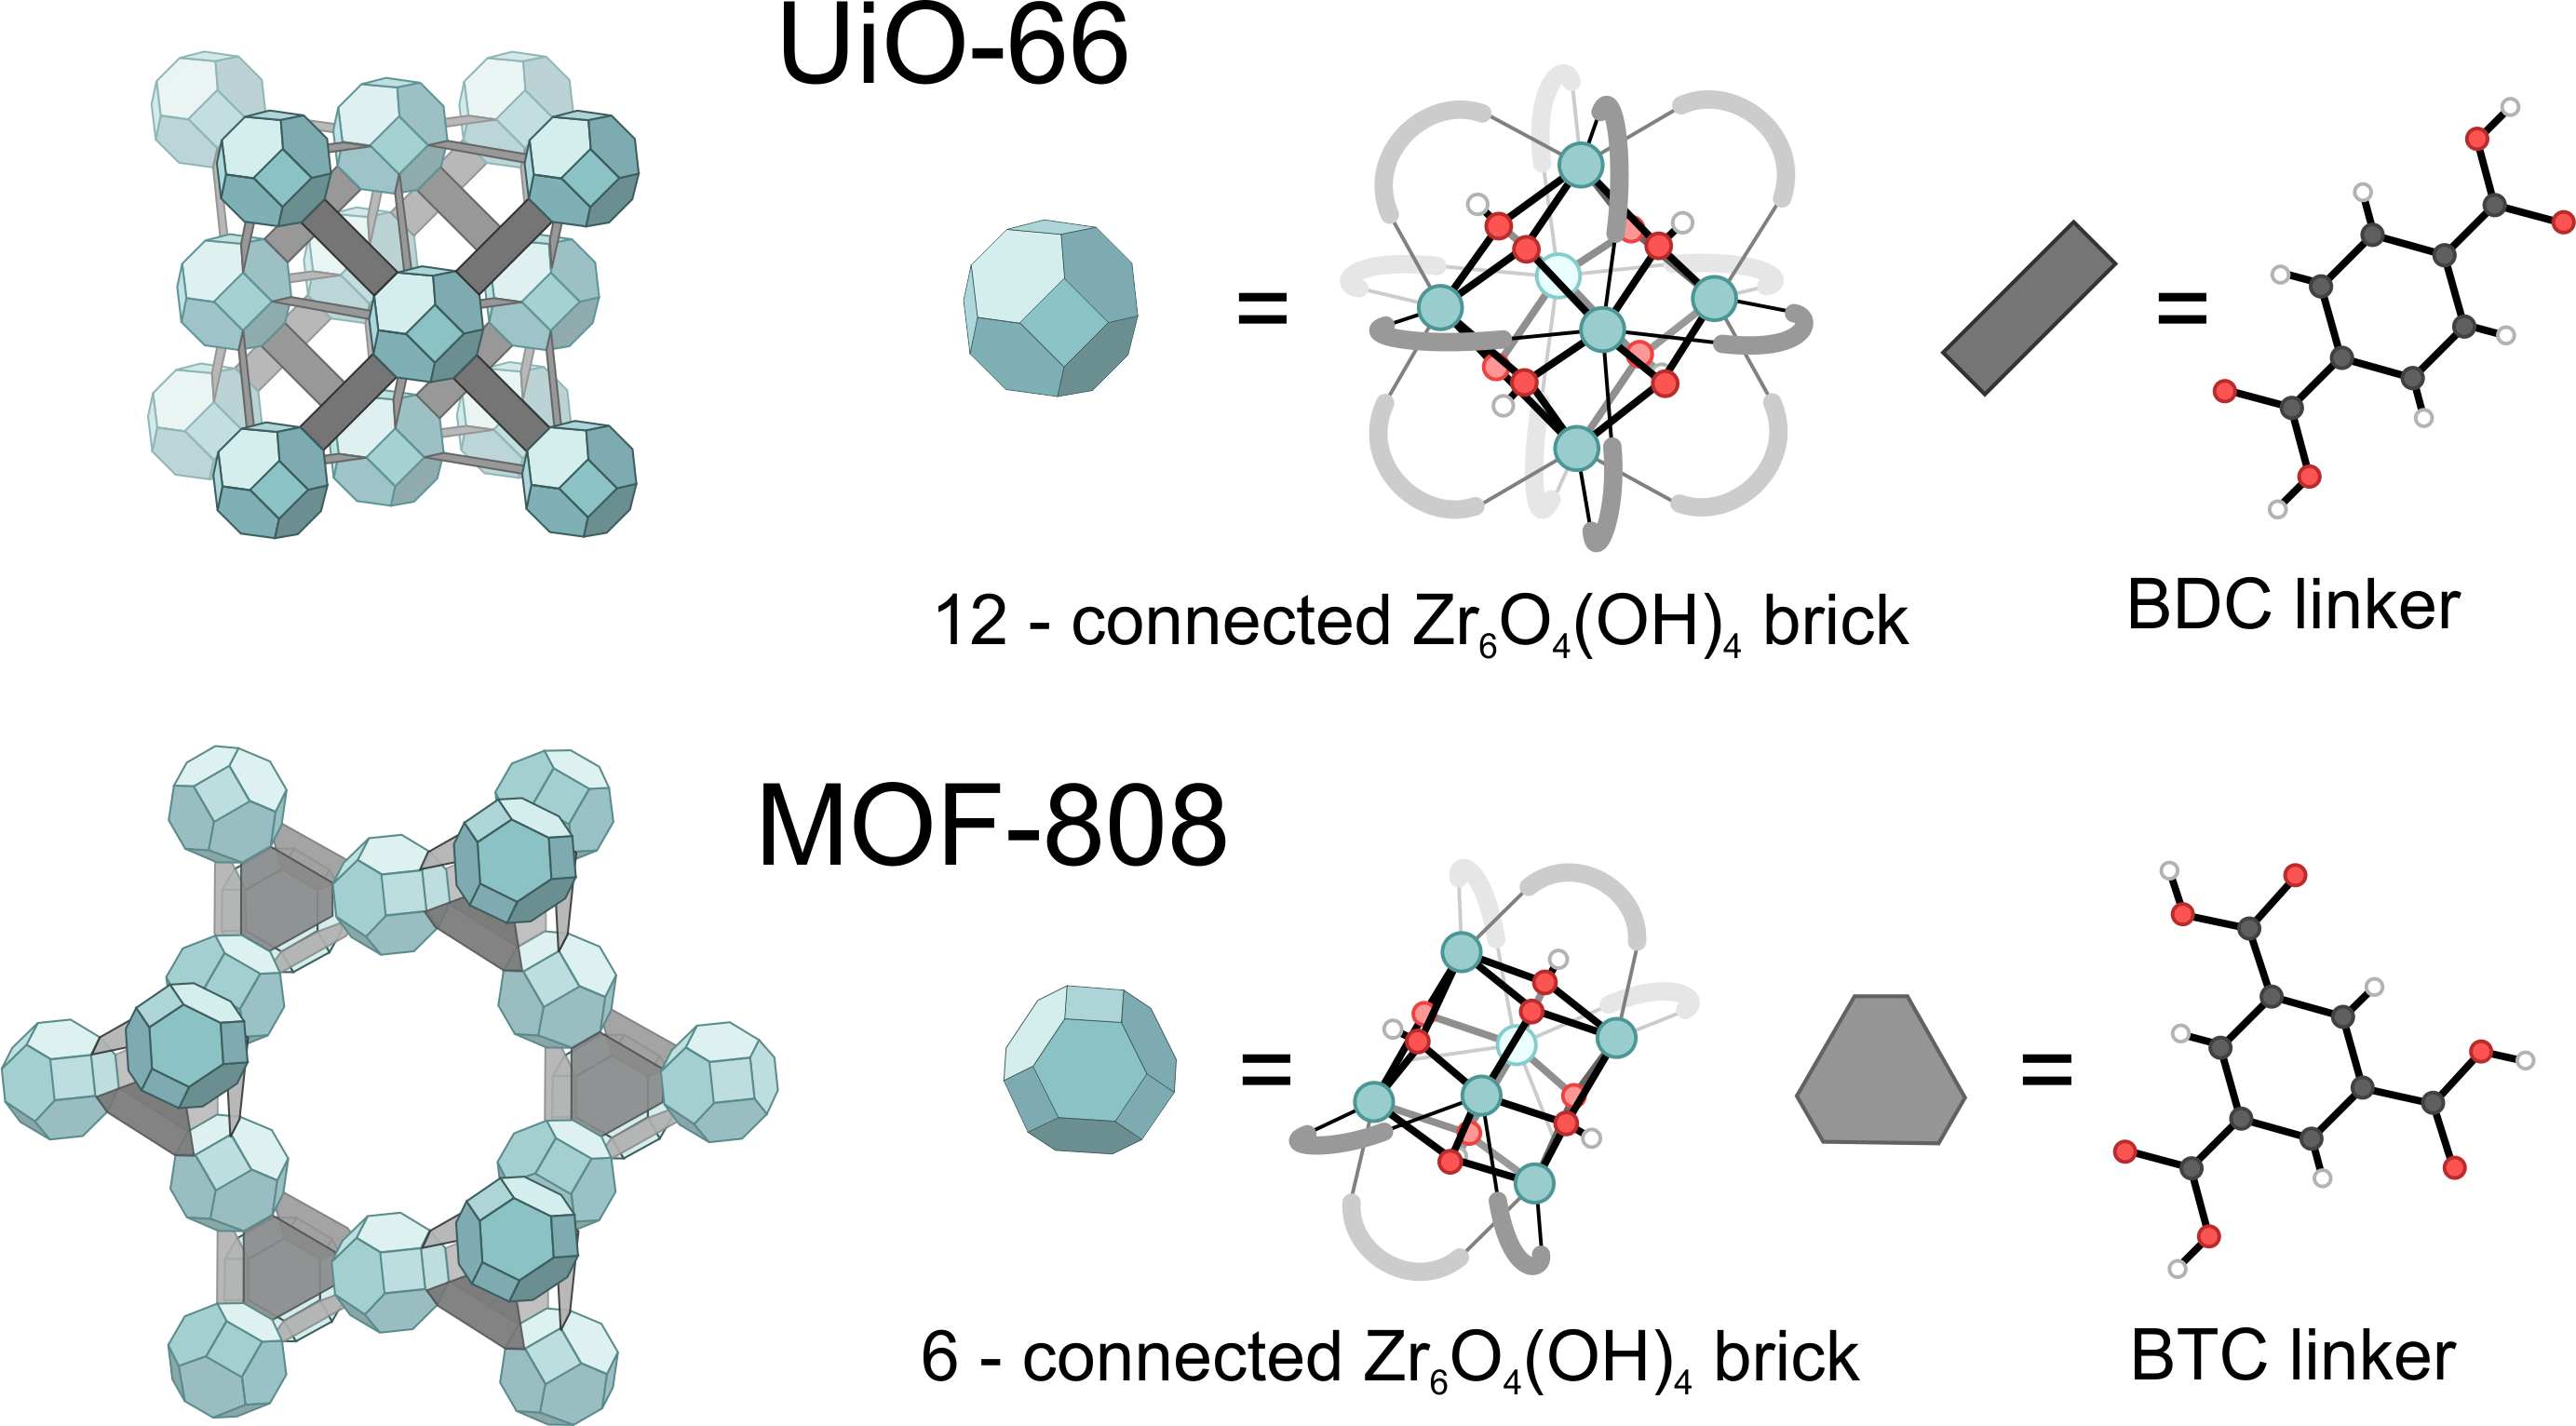
\includegraphics[width=1.0\textwidth]{Zr-MOFs}
	\caption{Structure of UiO--66 (top) and MOF--808 (bottom)}
	\label{fig:Zr-MOFs}
\end{figure}
%%
In general, to function at operating conditions, materials need to retain their thermal, mechanical and chemical stability at those conditions. For instance, mechanical stability is needed when compressing MOF in pellets or other shapes for industrial processes\cite{chapman2009pressure}, while chemical stability is crucial for any application, such as drug delivery, molecular separation, or catalysis\cite{horcajada2010porous}. Catalysis often also requires LISthermal stability, as the materials must be able to resist harsher conditions for certain processes such as in petrochemistry. 
However, the metal--ligand coordination bond that makes MOFs so tunable is also regarded as one of their main drawbacks\cite{keskin2010can, canivet2014water, kizzie2011effect}, as it is responsible for the lower structural stability when compared to already established nanoporous catalysts such as zeolites. For example, the first synthesized MOFs such as \ce{Cu2+} trimesate HKUST-1, or MOF-5, composed by \ce{Zn2+} clusters and BDC linkers were degraded by water even at mild conditions\cite{greathouse2006interaction, low2009virtual, kaye2007impact, decoste2013effect}. 
Recently, a class of robust MOFs have been synthesized showing an unprecedented stability\cite{furukawa2014water}. Zr--based MOFs\cite{bai2016zr} which exploit the robustness of the Zr--O bond, show an outstanding stability and are at present time one of the most studied classes of MOFs. Zirconium is an ubiquitous metal that is present in biological systems and has low toxicity, as well as limited cost. This makes these materials particularly promising for applications in catalysis, gas sorption, and drug delivery. The vast majority of these materials is characterized by Zr(IV) atoms in a high coordination state, which interact strongly with the oxygens of carboxylate linkers of various topology. These MOFs are characterized by a \ce{Zr6O4(OH)4} cluster in which each of the 6 zirconium atoms is connected to 4 oxygen atoms (two $\mu_3$--OH and two $\mu_3$--O), each of which is connected to three zirconium atoms, forming a polyhedron (Fig. \ref{fig:Zr-MOFs}). Each zirconium atom can in turn form 4 other bonds with ligands, accommodating up to 24 metal--ligand bonds per cluster. Each zirconium atom can therefore form a total of 8 coordination bonds in a square--antiprismatic geometry, yielding a rich range of possible structures that can be synthesized. The dual Lewis acid/base nature of the Zr--carboxylate bonds, along with the high metal oxidation state, gives rise to strong interactions between the SBUs, thus allowing processes such as PSM without compromising the stability of the structures. Different structures can be constructed with this SBU and different linker topology and connectivity ranging from 12, like in UiO--66, to 6 as in MOF--808 (see Fig. \ref{fig:Zr-MOFs}). These materials can further be functionalized by post synthetic modification. 
The stability of Zr--based MOFs is related to the connectivity between the inorganic and organic SBUs, as well as the number of zirconium--ligand bonds. However, open metal sites in these materials are present only when the connectivity of the linkers is less than 12. Zirconium atoms that remain undercoordinated in these materials are Lewis acid sites where reactants can adsorb and that can function as catalytic centers.

\subsection*{UiO--66}
The precursor of the whole class of Zr--based MOFs is the Zr--therephtalate based UiO--66, which was first synthesized at the Universiteit i Oslo by Lillerud and coworkers\cite{cavka2008new}. This material is characterized by an extremely high connectivity that gives rise to an exceptional structural stability, which makes UiO--66 one of the most widely investigated MOFs up to date. In this material, each \ce{Zr6} SBU is connected to 12 therephthalate (or benzenedicarboxylate (BDC)) linkers forming a cubic close packed structure with a space group F$\bar{\mathrm{m}}$3m, No. 225. In this structure there are two different cavities of octahedral and tetrahedral shape, with window sizes of 10 $\mathrm{\AA}$ and 25 $\mathrm{\AA}$, respectively. Each octahedral cage shares triangular windows with eight tetrahedral cages. 
This results in an extremely robust material which is stable up to 375$^{\circ}$C and in most solvents and pH conditions. Moreover, the \ce{Zr6O4(OH)4} bricks be reversibly dehydrated upon thermal treatment at temperatures above 300$^{\circ}$C. Up to two water molecules can be formed this way, yielding a \ce{Zr6O6} brick, where the zirconium atoms have a coordination of 7\cite{valenzano2011disclosing}. 
A whole family of isoreticular MOFs can be derived from UiO--66 by using linkers of different size, spanning from fumaric acid\cite{wissmann2012modulated} up to terphenyldicarboxylic acid\cite{schaate2011modulated}. Interpenetrated MOFs with UiO--66 topology have been also reported if longer linkers are used\cite{schaate2011porous}. Moreover, different functional groups can be appended to the phenyl rings, such as bromo, amino, nitro, or naphthalene. Garibay and Cohen showed that UiO--66--\ce{NH2} can be further modified to yield new functionalized frameworks \cite{garibay2010isoreticular}. Also the inorganic SBUs can be modified, for instance introducing 
titanium or hafnium\cite{kim2012postsynthetic}. The exceptional thermal and chemical stability of UiO--66 allows all these modifications of the structure, and for this reason, this material is often considered a perfect MOF archetype. 

\begin{figure}[!htbp]
	\centering
 	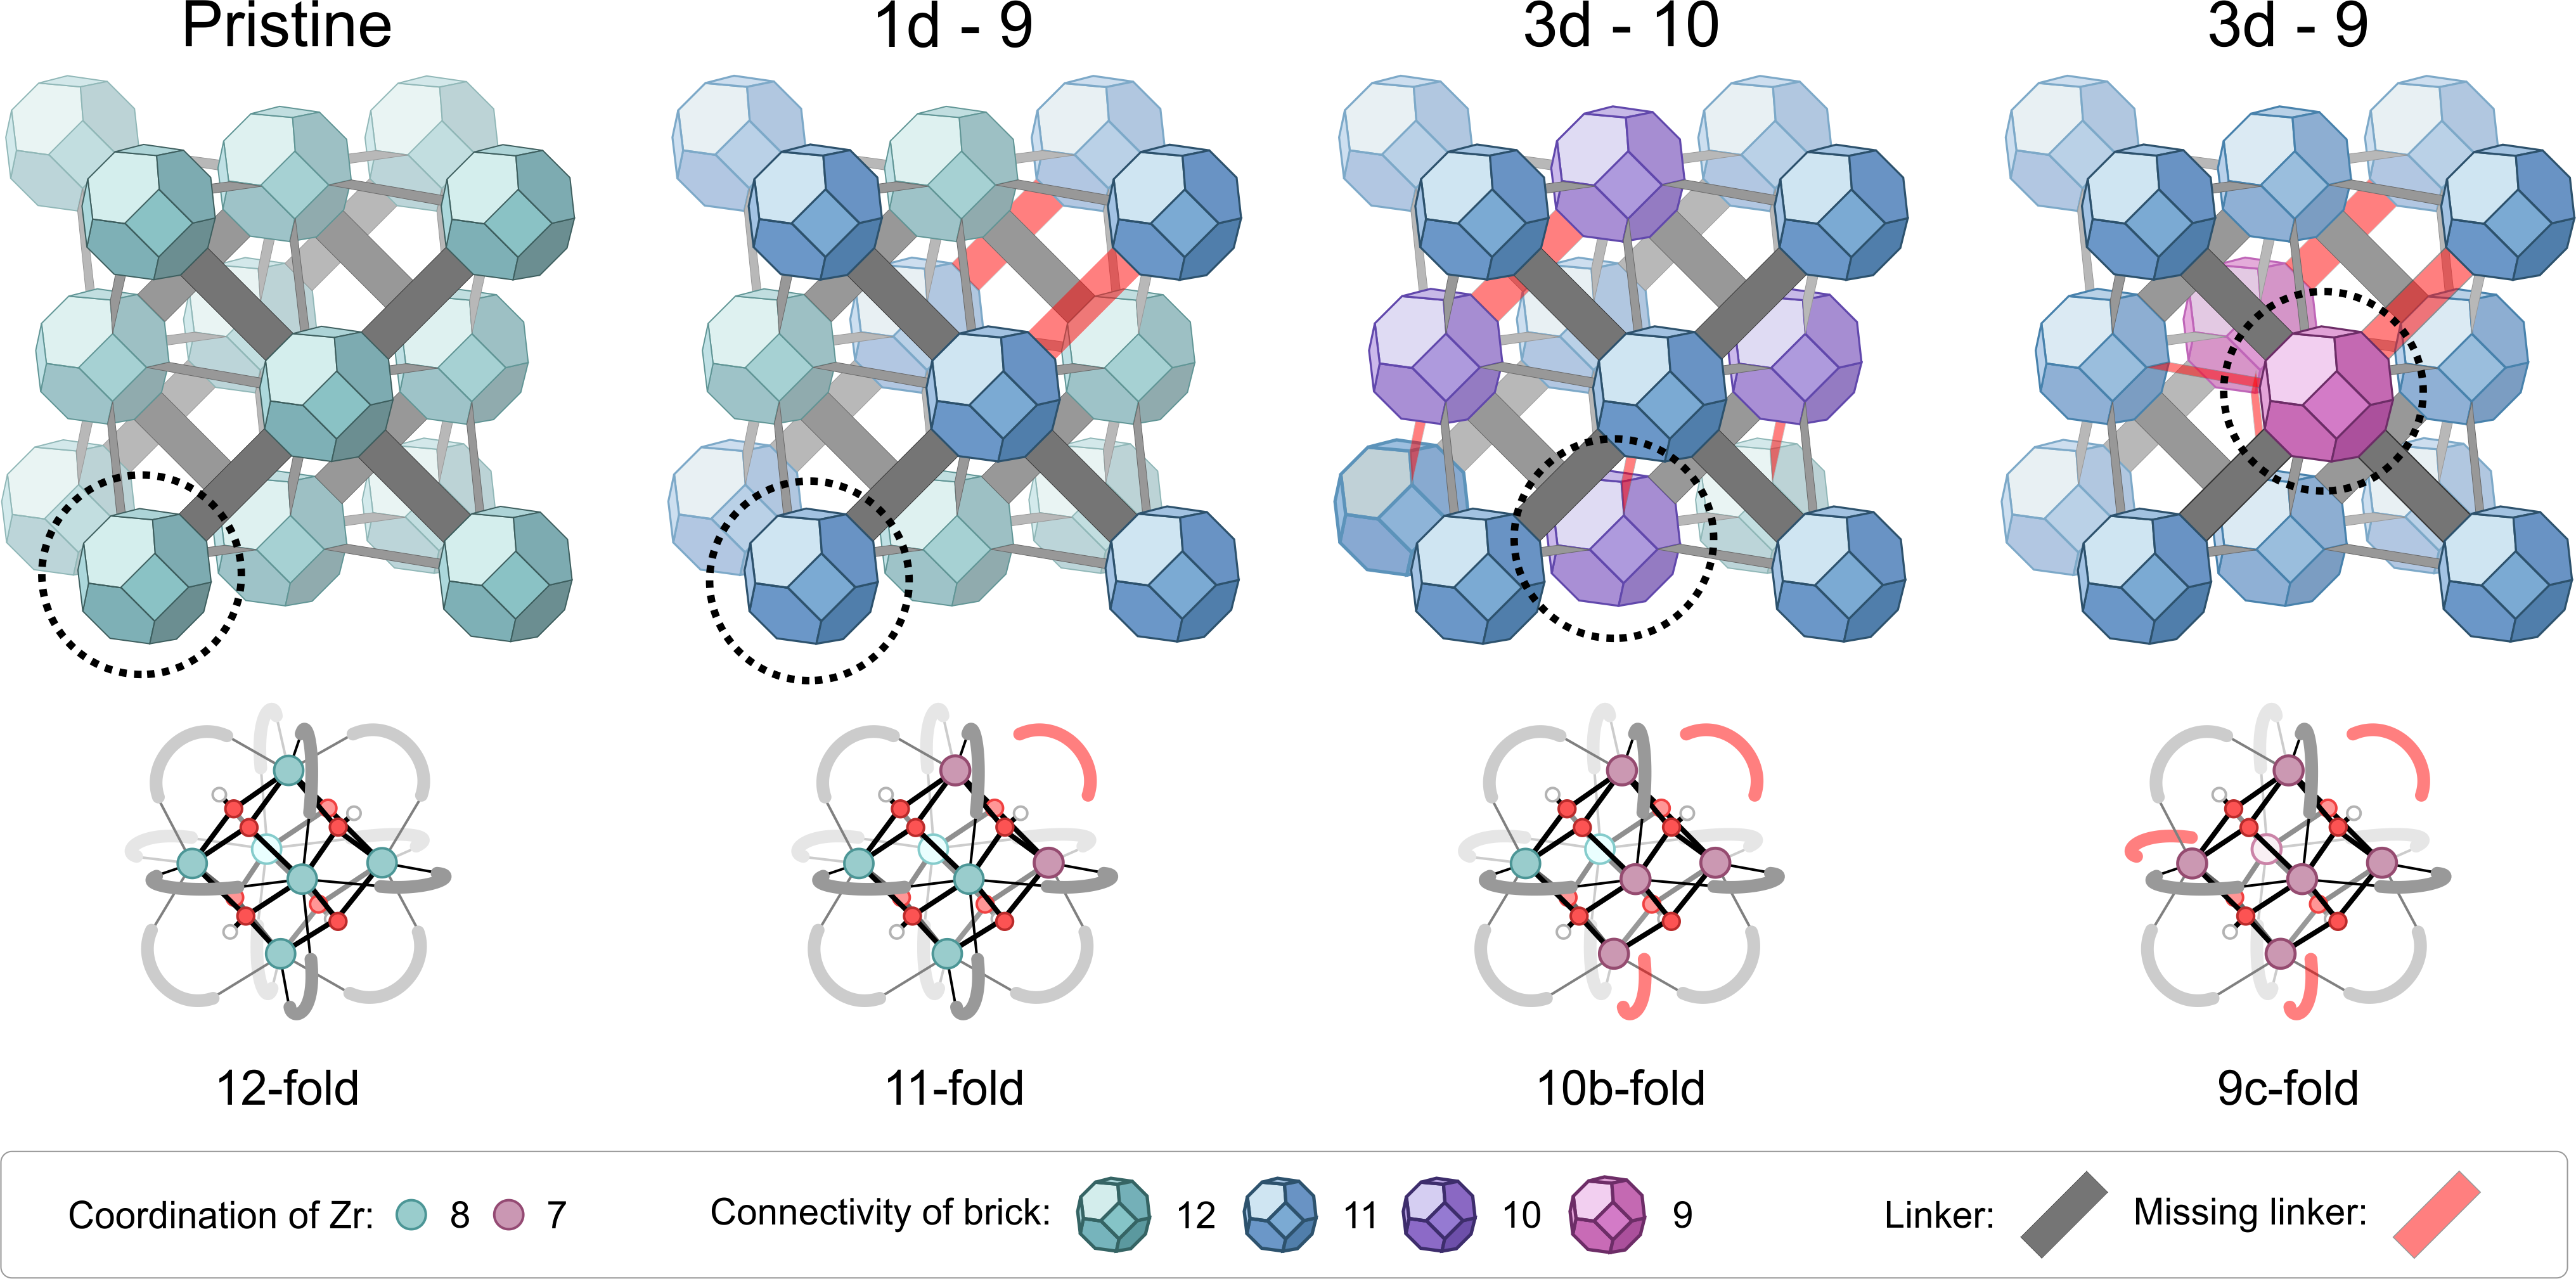
\includegraphics[width=1.0\textwidth]{defectivebricks}
	\caption{Defective UiO--66 unit cells with different number of missing linkers}
	\label{fig:defectivebricks}
\end{figure}

\subsubsection*{Defects}
%chap 11 of book from Garcia
In theory, the perfect crystalline UiO--66 structure, where every zirconium atom is 8--fold coordinated, does not possess undercoodinated Lewis acid sites available for catalysis. However, it became clear that the synthesized UiO--66 showed a behavior that deviated from the theory and pointed towards the presence of defective sites, such as symmetry--forbidden reflections in the PXRD pattern, metal--linker ration obtained by thermogravimetric analysis (TGA), higher than expected surface area, appearance of O--H stretching bands in the FTIR spectrum etc. \cite{shearer2014tuned, valenzano2011disclosing}. It has been generally accepted that the material contains defects in the form of missing linkers or clusters, and that these are not only naturally occurring during synthesis, but their number can easily be tuned by adapting the synthesis conditions, such as temperature and presence of modulator\cite{wu2013unusual, shearer2016defect}. A decrease in the connectivity in the structure will naturally lead to a decrease in stability of the material, but the extremely high connectivity of UiO--66 allows the presence of numerous missing linkers or cluster without loss of crystallinity\cite{rogge2016thermodynamic}. 
These defective sites in MOFs can be either point vacancies (such as missing linkers or clusters) or extended ones such as in the case of a surface \cite{sholl2015defects}. 


The physical properties of defective UiO--66 differ according to the number of defects and their location, as has been extensively studied both theoretically and experimentally. The beneficial role of defects in UiO--66 has been explored in many applications such as gas storage and separation\cite{wu2013unusual, ren2014modulated}, sensing\cite{stassen2016towards}, drug delivery\cite{cunha2013rationale} and catalysis\cite{vermoortele2013synthesis, rogge2017metal}. The inherent linker vacancies in UiO--66 bring unsaturated zirconium Lewis acid sites and at the same time enable the reactants accessibility to the sites, increasing the pore size. 
\td{The number of defects can be measured by ..}

\subsubsection*{Active sites for catalysis on UiO--66}
One of the breakthroughs of MOF research was the discovery that UiO--66 could contain a high number of open metal sites. As reported earlier, active sites for catalysis in UiO--66 and other Zr--MOFs are present when the zirconium connectivity is decreased from its equilibrium value of 8. 
%active sites by defects
A first way to obtain coordinatively unsaturated zirconium sites is by creation of defects, in the form of missing linkers or clusters. The synthesis of defective UiO--66 can be performed via modulators such as formic acid or trifluoroacetic acid (TFA), that are competing with BDC linkers in binding to the inorganic SBU. 
Vermoortele et al. first showed in a dual computational--experimental study that the Lewis catalyzed cyclization of citronellal can only be done on UiO--66 in case of missing linkers\cite{vermoortele2012electronic}. For Meerwein reduction, another Lewis catalyzed reaction, the catalytic activity of UiO--66 could be significantly increased by making use of TFA, that introduced a large number of linker vacancies. Additionally, the non-modulated material that contained only a small number of defects showed nearly no catalytic activity\cite{vermoortele2013synthesis}. 

It is known that on the defect site, different defect coordinating species such as water can be adsorbed. These species can be removed by thermal activation at T$>$200$^{\circ}$C, giving zirconium open metal sites for reaction. 



UiO--66 can be hydrolized \cite{decoste2013stability}
% active sites by dehydration
The material can be reversibly dehydrated,

\begin{figure}[!htbp]
	\centering
 	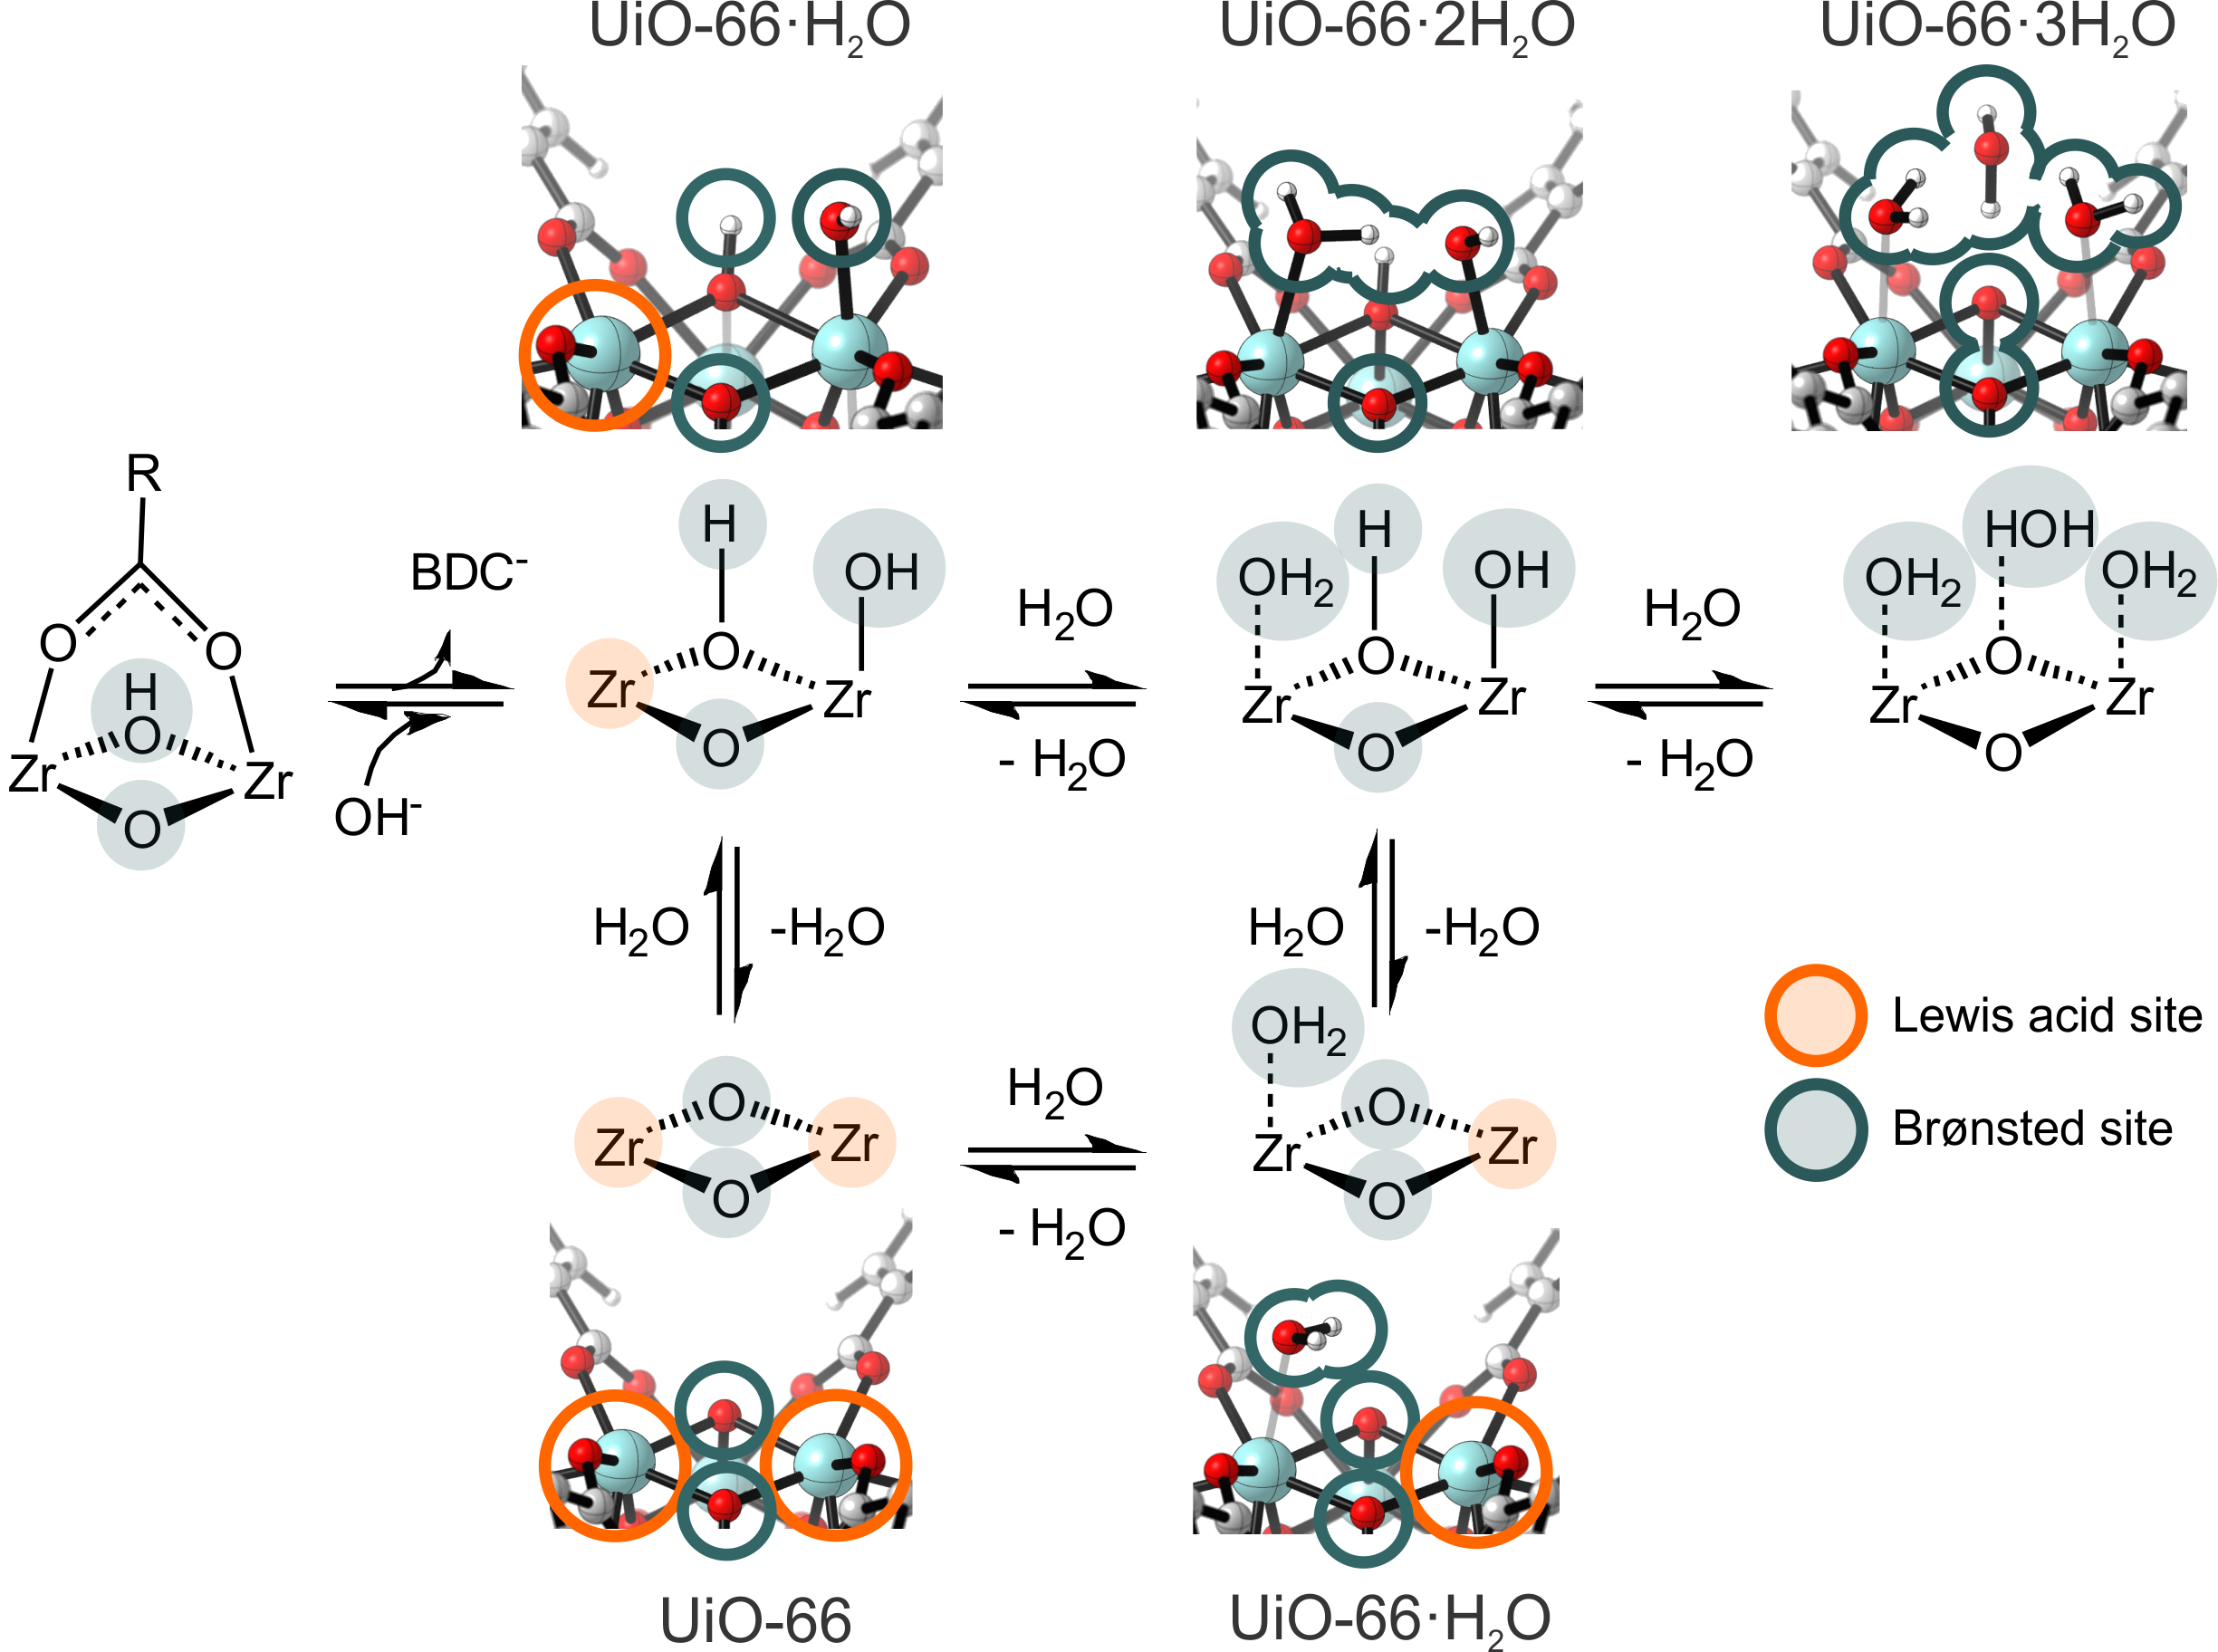
\includegraphics[width=1.0\textwidth]{bronsted-lewis-uio}
	\caption{Lewis and Br\o{}nsted site when a linker is removed from the UiO--66 zirconium brick}
	\label{fig:bronsted-lewis-uio}
\end{figure}

\subsection*{Outline and goal of the thesis}
In this chapter, the characteristics of MOFs that make them appealing as catalysts have been shown, as well as the current challenges. The properties of catalytically active sites on defective UiO--66 and MOF--808 were studied by means of molecular modeling techniques. Molecular modeling can give fundamental insight into the properties of MOFs, and at present time a plethora of different techniques are available for this purpose. To model processes in MOFs, knowledge of both power and limitations of these methods and experimental insight into the scientific question are required to find the appropriate combination of techniques.\\\\
This PhD thesis is organized as follows:
\begin{itemize}
\item In Chapter 2, a theoretical overview of the state of the art modeling techniques is given. Particular attention is drawn on how these techniques can be applied in the case of MOF materials to obtain insight into structural and catalytic properties at operating conditions.
\item In Chapter 3, the main results of this PhD thesis are summarized. The links between theory and experiment are highlighted throughout the chapter. All results are the result of fruitful collaborations and have been published in international peer--reviewed journals. 
\item In Chapter 4, the main conclusions of this thesis work, as well as perspectives on future research are given.
\end{itemize}




%
%%% Introduction
%%%%%%%%%%%%%%%%
%Over the last two decades, a new class of solid--state materials called porous functional materials, have become an
%object of intense study in the field of chemistry and materials science. They
%can be found in different fields in industry and are at the heart of many
%technological processes.
%The interest which has been devoted to these materials mainly arises from their potential to interact with ions, atoms and molecules not only at the surface, but also throughout the bulk of the material. High surface area, excellent accessibility to active sites, improved diffusion and mass transport are some of the outstanding properties which are typical for porous materials \cite{Davis2002, Perego2013}. It should not surprise that the traditional applications of porous solids include adsorption and catalysis, which benefit from the high order and porosity that can be reached in these materials. Porous materials can have different properties based on the diameter of their pores, which can be divided in different classes. According to the International Union of Pure and Applied Chemistry (IUPAC), micropores have a pore size diameter smaller than 2 nm, those in the range of 2 nm to 50 nm are designated mesopores, and those with diameters wider than 50 nm are macropores. The need to generate homogeneity within the distribution of sizes, shapes and volumes of the void spaces in porous materials has steadily increased over recent years because it can lead to superior application properties of technological importance \cite{Sun2016, Davis2002}. For functional porous materials, in addition to the pore space, the type and arrangement of atoms in the solid creating that space can also impact their properties to a large extent. The most appealing porous materials which have continuously attracted the interest of the scientific community over the years include zeolites and metal--organic frameworks (MOFs) (Figure \ref{fig:Figure intro}) \cite{Liang2017}. Despite their common features, they possess distinct differences which determine their range of applications, and particularly their role in catalysis. Within this thesis, major attention will be focused on MOFs although some selected applications were also performed with zeolites.
%In what follows a short classification of these materials will be given.  
%
%\begin{figure}[!h] 
% 	\centering
%	\includegraphics[width=1.0\textwidth]{Figure_intro}
%	\caption{Number of yearly publications, up to 2017, containing the concepts
%	'MOF*' and 'zeolite*' as indicated by Web of Science. Periodic representations
%	of H--ZSM--5 and MOF--5 are shown.}
%	\label{fig:Figure intro}
%\end{figure}
%
%
%\section{Zeolites}
%Zeolites represent a major group of crystalline microporous materials, which are
%formed naturally in association with volcanic activity, but can also be
%synthesized in a wide range of structures. They are aluminosilicates composed
%of corner--sharing \ce{SiO4} and \ce{AlO4} tetrahedra, which leads to 3--D
%four--connected frameworks. Whenever tetravalent Si is substituted by trivalent
%atoms such as Al, electron--neutrality needs to be retained by 
%incorporation of charge balancing cations, which are located as the extra framework sites in the channels and cages. A whole plethora of cationic species such as alkali and alkaline earth, transition
%metal and lanthanide cations can be used creating Lewis acid sites. A very
%particular case is compensation by
%protons which bond to the bridging oxygen atoms leading to the formation of
%strongly acidic Br\o{}nsted sites, which have a key role in zeolite catalyzed
%reactions. Other tetrahedrally coordinated atoms
%like Ge, B, P and Ti can also be incorporated into the framework to complement the
%zeolite family \cite{Nagy1998, Cejka2010, VanSpeybroeck2015}. The
%Structure Commission of the International Zeolite Association (IZA--SC)
%has now officially recognized more than two hundred types of zeolite frameworks
%which have different size, shape, and channels connectivity \cite{Database}.
%Since 1960s, due to their exceptional stability zeolites have been used as heterogeneous catalysts under harsh conditions. Among the
%plethora of known zeolite structures, ZSM--5 with MFI topology has received a
%lot of attention due to its efficient performance in chemical
%industry \cite{Liang2017}. Together with FAU, BEA, MOR and FER topologies, it
%belongs to the 'Big Five' zeolite structures that are most commonly used in
%industrial applications \cite{VanSpeybroeck2015}. The H--ZSM--5 material
%consists of two types of channels, sinusoidal and straight channels, which are oriented
%perpendicularly to each other and make up a 3--D framework of a medium pore size
%(Figure \ref{fig:Figure intro}, H--ZSM--5). The H--ZSM--5 possesses Br\o{}nsted
%acid sites, and due to its exceptional synergy between hydrothermal stability,
%activity and selectivity, it is one of the most successful industrial
%heterogeneous catalysts with various applications such as methanol--to--olefins
%(MTO) and alkene cracking \cite{Olsbye2012, Lefevere2014}. In both processes alkenes play a crucial role but their adsorption is almost impossible to follow on a purely experimental basis as these hydrocarbons are highly reactive even at low temperature. To gain insight into the nature of the adsorbed complexes and intermediates at operating conditions the study on the adsorption
%behavior of linear pentenes on H--ZSM--5 was performed in \textbf{Paper VI}
%within this PhD thesis.
%
%
%\section{MOFs}
%Another class of crystalline porous materials, which has drawn increasing
%attention of the scientific community consists of hybrid frameworks. Even
%though, the first reports about MOFs or, broadly speaking, on coordination
%polymers date from the late 1950s and early 1960s \cite{Knobloch1959,
%Berlin1960, Kubo1960, Block1962, Tomic1965, Kinoshita1959}, only in the end of
%the last century these materials were rediscovered by four pioneering groups:
%Robson \cite{Hoskins1990, Batten1995}, Kitagawa \cite{Kitagawa1991,
%Kitagawa1993}, Yaghi \cite{Yaghi1995} and F\'erey \cite{Riou1998}. MOFs in
%contrast to solely inorganic zeolites are truly hybrid materials built up regularly from organic and inorganic building blocks.
%In these materials, metal ions or clusters are connected by multitopic organic molecules to form
%1--, 2-- or 3--D pore structures.
%In principle, all the transition metals and a broad variety of organic linkers
%can be used in the synthesis. A very particular characteristic of the hybrid
%materials is an exceptionally large variability in composition, porosity and
%functionality which makes them different from the classical inorganic porous
%materials and leads to more than ten thousand frameworks which have already been
%synthesised.
%The structural beauty of MOFs arises from the endless number of highly ordered structures which can in general be synthesized from their
%building blocks, which can in turn be further tuned by means of postsynthetic
%modification. These materials possess specific surface area and pore volumes
%which leads to very high adsorption capacity and much higher porosity than that
%of zeolites \cite{Llabres2013}. A remarkable property of some MOFs, which is not
%found in other porous materials is the flexible response to the presence of guest
%molecules and external stimuli. The so called breathing MOFs or soft porous
%crystals have the ability to undergo structural deformations while retaining
%their stability upon exposure to external stimuli \cite{Horike2009,
%Schneemann2014}. The breathing behavior of MOFs is characterized by structural
%transformations going from large--pore to small--pore and \textit{vice versa},
%while the materials retain their crystallinity. Typically, the deformation
%occurs at the metal--linker (M--L) coordination, but without any bond cleavage in the solid. The M--L coordination bonds are
%generally weaker than covalent bonds, and are kinetically the most labile parts in
%MOFs \cite{Bennett2017, Morris2017}. The strength of the M--L bond is determined
%by the combined properties of metal species and connecting ligands, which is in
%line with the Lewis acid--base coordination chemistry concept. Whereas
%first--generation MOFs suffered from limited stability, especially when compared
%to industrially relevant zeolites, in recent years, a whole series of robust MOF
%structures has been constructed, enabling the expansion of their
%applications \cite{Burtch2014, Bai2016, Liu2017}. Within this respect, the
%Zr--terephthalate UiO--66 has received
%enormous attention due to its exceptional thermal, mechanical and chemical
%stability \cite{Cavka2008, Valenzano2011, Wu2013}, and its application in
%heterogeneous catalysis is the main topic of this PhD thesis.
%
%
%\section{Defects -- origin of highly active catalysts}
%\label{sec:defects} 
% \begin{quotation}
%Crystals are like people: it is the defects in them
%which tend to make them interesting! -- Colin Humphreys --
% \end{quotation}
%\npar
%Structural disorders and defects of various nature are crucial characteristics
%of porous solids and recently it has become evident that defects, disorder and structural heterogeneity are key
%attributes while estimating and investigating the structure and activity of
%MOFs. Over the past decades, the controlled modification of zeolites has proven
%to be decisive for their technological applications. 
%In as--synthesized zeolites,
%acid strength, elemental composition, pore texture or stability are often
%insufficient for the harsh conditions used in industry. However, postsynthetic
%methods which are available to tailor the composition, stability and nature of
%active sites in zeolites provide novel opportunities for catalytic or sorption
%applications. Such postsynthetic zeolite modifications may lead to selective
%cleavage or formation of metal--oxygen bonds, which in most cases is
%irreversible. In comparison, the formation of M--L coordinative
%bonds in MOFs is reversible, and therefore, the postsythetic modifications in MOFs offer an even higher degree of defect engineering potential.
%In many cases even the most carefully synthesized MOFs accommodate a diversity
%of defects which in many applications can control the overall performance of a material.
%For this reason, an accurate characterization and understanding of defects and their effect in
%MOFs are essential for further progress in the field of industrially relevant
%applications of these materials. Defects in MOFs can arise from multiple
%reasons.
%Linkers or metal nodes vacancies are classified as local defects, and
%can be distinguished from line defects which are formed by
%dislocations, planar defects (grain boundaries) and voids which form
%empty spaces in the crystal (Figure \ref{fig:defects}). 
%
%\begin{figure}[!h] 
% 	\centering
%	\includegraphics[width=1.0\textwidth]{defects}
%	\caption[The definition of defects: the missing and incorrectly located atoms
%generate vacancies and dislocations in materials.]{The definition of defects:
%the missing and incorrectly located atoms generate vacancies and dislocations in
%materials \cite{Fang2015}. Adapted with permission from Wiley-VCH Verlag,
%copyright 2015.}
%	\label{fig:defects}
%\end{figure}
%\npar
%In this respect, Sholl
%\textit{et al.}\cite{Sholl2015} classified disorders in MOFs, simply distinguishing point defects which are crystal vacancies of vacant ligands and vacant metal centers,
%from extended defects which are associated with 1-- or 2--D imperfections in the
%crystal structure. Another type of classification was recently introduced by Fang \textit{et al.}\cite{Fang2015} 
%in which defects were distinguished based on the source of their origin. 
%Firstly, inherent defects were defined as structural deformations which can occur without targeted engineering during synthesis under regular synthetic conditions. 
%Secondly, the great modularity of MOFs gave rise to a class of engineered defects which is generated from intentional 
%creation of various types of imperfections for desired purposes.
%The existence of defects in MOFs affects the chemical nature of
%the pore surface altering the host--guest interactions, and can have a significant positive impact on applications such as catalysis.
%
%
%\subsection*{MOFs as single site catalysts}
%Catalysis can be easily located at the heart of chemistry as all chemical
%reactions involve forming and breaking of chemical bonds, which can be
%more efficiently and selectively done with the use of a catalyst. A very specific
%characteristic of homogeneous catalysts is the presence of a single active
%site. From this point of view, zeolites and MOFs are very attractive, since they
%possess catalytic well--defined, isolated single--sites usually in the form of
%defects. In light of the synthetic and
%postsynthetic modifications, five theoretically different types of active sites
%have been proposed to design MOFs for catalytic application, as schematically
%shown in Figure \ref{fig:active_sites}
%\cite{Chughtai2015,Corma2010,Lee2009,Li2016,Liu2014,Rogge2017}.
%
%\begin{figure}[!h]
%	\centering
%	\includegraphics[width=1.0\textwidth]{active_sites}
%	\caption[Classification of the different positions in porous framework
%	materials where single--site catalytic reactions can take place. The inorganic
%	nodes are indicated with cyan spheres, whereas the structure-defining ligands
%	are indicated in grey. Possible terminating ligands at the inorganic nodes are not indicated, as they do not contribute to the topology of the material.]{Classification of the different positions in porous framework
%	materials where single--site catalytic reactions can take place. The inorganic
%	nodes are indicated with cyan spheres, whereas the structure-defining ligands
%	are indicated in grey. Possible terminating ligands at the inorganic nodes are not indicated, as they do not contribute to the topology of the material. Adapted
%from Ref. \cite{Rogge2017}.}
%	\label{fig:active_sites}
%\end{figure}
%\npar
%\newpage
%The activity within type I catalysts is directly related to metal centers with
%an unsaturated coordination environment. These sites are commonly specified as
%open metal sites or coordinatively unsaturated sites. In this case, the metal
%has a dual role of a structural building component and an active site. Some MOFs
%made from fully coordinated inorganic nodes had at first sight a lack of active
%sites. Several strategies were applied to deliberately create active sites
%by introducing desired defects on the material \cite{Fang2015}. Type I includes
%generally catalysis at open metal sites created by structural defects. The coordinatively unsaturated sites can be terminated by catalytically active ligands. In MOFs with linker vacancies, the coordinatively unsaturated
%metals can be hydroxylated and depending on substrates may hold Br\o{}nsted or
%Lewis acidity (Figure \ref{fig:active_sites}, Type I).
%Within type II catalyst, the activity is associated with a metal
%embedded in a porphyrin--based ligand. These MOFs contain two different types of
%metals so that one gives rise to the catalytic activity while the role of the
%second metal is limited to structural function in the composition of the material.
%The nature of the catalytic site may be modified by postsynthetically tuning
%the metal atom at the center of the porphyrin ligand.
%Type III active sites based on covalently anchored functional groups on the
%organic linker. These catalytically active functional groups might be present
%during synthesis or added postsynthetically. The terminating groups
%do not connect different building blocks of the material framework, which 
%differentiate them from metalloporphyrins.
%Within type IV catalysts, the external surface of the material is considered as
%it has been reported that in some cases it might be the most defective place in
%the structure for the location of the reactive sites \cite{Chizallet2010a,
%Chizallet2010b}. The last category V includes the nanoparticles which are encapsulated in the
%framework cavities by host--guest interactions \cite{Dhakshinamoorthy2012,
%Juan-Alcaniz2013}. In this case the framework supplies the physical space for
%catalytically active sites, although none of the components of the building
%metal framework is directly involved in the catalysis. A thorough description of
%the active sites of type I, II and III is presented in \textbf{Paper IX} of this
%thesis \cite{Rogge2017}.
%
%
%\section{MOFs stability}
%The construction of thousands of well--established MOFs structures with a
%broad range of topologies, pore size and functionalities, has led to
%the study of many applications. Regardless of the method applied to introduce
%the active sites in MOFs, in order to be used in potential industrial applications, the materials
%have to be stable under catalytic conditions.
%In this respect, the necessity to
%engender MOFs which possess mechanical, thermal and chemical stability
%has become a key research focus. Theoretically, the understanding
%of the degradation mechanism is of paramount importance in the discovery of
%stable materials and in the prediction of their behavior under reaction
%conditions.
%Due to the presence of coordinative bonds in MOFs, the stability in general has been typically recognized as problematic, especially
%when compared to zeolites, constructed with strong covalent bonds. However, as
%the number and diversity of MOF materials have grown significantly, their stability has also
%substantially increased, giving rise to a whole plethora of
%mechanically, chemically and thermally stable frameworks \cite{Howarth2016}.
%\newpage
%\section{UiO--66 as a prototype of \ce{Zr6}--containing MOFs}
%\label{sec:UiO-66}
%Among the broad family of MOFs, especially the \ce{Zr6}--based MOFs have
%received a lot of attention from scientists, as they reveal rich structure
%types, intriguing properties and functions which make them some of the most
%promising MOF materials for practical applications \cite{Bai2016}. The
%breakthrough in the field is seen in 2008 with the discovery of the Zr--terephthalate UiO--66, which can be
%considered as the prototype of this subfamily of MOFs \cite{Cavka2008}. In the
%pristine structure of UiO--66 each Zr secondary building unit (SBU)
%\ce{Zr6O4(OH)4} is coordinated to twelve terephthalate linkers to form a 3--D porous framework (Figure \ref{fig:UiO-66}). The SBU consists
%of six \ce{Zr4+} cations which are located on the vertices of an octahedron, on
%which four bridging \ce{{\textmu}3}--oxygens and four \ce{{\textmu}3}--hydroxyl
%groups are capped alternatively in the eight faces. Each carboxylate linker is
%connected to two Zr atoms from the same SBU bridging the edges of \ce{Zr6} octahedron. The
%structure exhibits superior stability, which can be directly traced back to the
%inherent composition of the framework \cite{Valenzano2011, Wu2013}. In the case
%of UiO--66, the high oxidation state of Zr ions and bond polarizability leads to
%a more strongly binding coordination complex and gives rise to a remarkable
%thermal and chemical stability of the material. Furthermore, the relative
%weakness of the M--L coordination bond should be seen as an advantage in the
%activation processes to which MOFs, and in particular the archetypal UiO--66 is
%examined \cite{Burtch2014, Morris2017}. Recently, undeniable evidence was given
%that the inorganic brick, with its high degree of coordination within the
%UiO--66 material, is much more dynamic than originally believed
%\cite{Nishida2014, Cohen2017, Kim2012, Kim2012a}. The material maintains its structural integrity after being exposed to activation processes such as modulation, dehydration or linker exchange yet changing the coordination around the metal center by temporarily breaking M--L bond as shown in \textbf{Paper III} and which will be further discussed in Chapter 3 of this thesis.
%
%\begin{figure}[!h]
%	\centering
%	\includegraphics[width=1.0\textwidth]{UiO-66}
%	\caption[Schematic representation of the UiO--66 structure with possible
%	configurations of the bricks that give rise to coordinatively unsaturated Zr
%	atoms. The colors indicate the coordination of the Zr atoms.]{Schematic
%	representation of the UiO--66 structure with possible configurations of the bricks that give rise to coordinatively unsaturated Zr
%	atoms. The colors indicate the coordination of the Zr atoms. Reprinted from
%	Ref. \cite{Hajek2018} with permission of the Royal Society of Chemistry,
%	copyright 2018.}
%	\label{fig:UiO-66}
%\end{figure}
%
%\newpage
%\subsection*{Activation by ligand removal}
%In view of the potential applications of UiO--66, the aspect of defect
%engineering has drawn a lot of attention. It was quickly discovered that the
%theoretical maximum number of twelve linkers per cluster could almost never been
%reached \cite{Valenzano2011,Shearer2014}. The study of the thermogravimetric
%analysis profiles tends to show that in most cases the average number of linkers surrounding each metal cluster varies between eleven and eight
%and strongly relies on the applied synthesis parameters (Figure \ref{fig:UiO-66}
%missing linker).
%A tunable composition of UiO--66 and the existence of linker defects leads to
%greatly improved porosity, adsorption properties and catalytic activity by means of the presence of accessible metal sites with a low coordination number which
%are Lewis acid sites \cite{Wu2013, Shearer2014, Vermoortele2013,Vandichel2015,
%Liu2016}. Ling and Slater revealed that in the aquatic environment, charge
%balancing hydroxide anions and water are bonded to coordinatively unsaturated Zr
%sites creating potential Br\o{}nsted base and acid centers \cite{Ling2016}.
%Similar conclusions were drawn in the framework of this thesis and are also
%discussed in \textbf{Paper II} and \textbf{Paper VII}.
%Moreover, the coordinatively unsaturated Lewis acid sites can be reaccomplished
%by the removal of water or other labile ligands which usually are solvent molecules, such as alcohols or dimethylformamide. 
%
%
%\subsection*{Activation by dehydration}
%Another process which can change the coordination environment of a metal is
%dehydration. A remarkable property of UiO--66 is the ability to be dehydrated
%reversibly. Experimentally the dehydration and rehydration process of the
%inorganic UiO--66 brick was studied using \textit{in situ} infrared (IR) spectroscopy and gravimetric
%characterization techniques (TG--DSC), proving that the reaction is
%reversible \cite{Shearer2013}. The dehydration of the defect--free UiO--66
%material involves the removal of
%two water molecules per inorganic brick, which starts at 523 K and is completed
%at 573 K. The dehydration process begins with the first water removal and
%results in a \ce{Zr6O5(OH)2} brick, where the coordination number of three Zr
%atoms decreases from 8 to 7 (Figure \ref{fig:UiO-66}, partly dehydrated brick). The fully dehydrated brick results in a distorted composition of \ce{Zr6O6} with Zr coordination numbers
%varying from 8 to 6 (Figure \ref{fig:UiO-66}, fully dehydrated brick). Moreover,
%a rehydration reaction restores the material to its initial structure maintaining the robustness of the brick which was confirmed by powder X--Ray diffraction (PXRD) patterns, \textit{in situ} diffuse reflectance infrared Fourier transform
%(DRIFT) spectra and TG--DSC \cite{Shearer2013, Valenzano2011}. Within this
%thesis, \textbf{Paper II} gives a comprehensive overview of the dehydration
%mechanism of UiO--66 with different defectivity \cite{Vandichel2016}. The
%position of linker defects in UiO--66 does not affect the reaction mechanism and requires the same energy at
%atmospheric pressure and temperature of 573 K. The mechanism of dehydration
%process is characterized by two crucial transition states.
%The first one corresponds to the decoordination of both, terephthalate linker
%and hydroxyl group, while the second describes the protonation of a dangling
%hydroxyl group by another available \ce{{\textmu}3}--OH to form water. The endothermic
%nature of dehydration was proved both experimentally and
%theoretically \cite{Shearer2013, Vandichel2016}.
%
%
%\subsection*{Activation by linker and cation exchange}
%The inherent dynamic behavior of robust MOFs and reversible chemistry of the
%M--L bond has a direct impact on the ability to subject the materials to a
%postsynthetic exchange processes. In the framework of UiO--66, pure BDC linkers
%were replaced by functionalized ones without compromising the crystallinity or
%porosity of the material \cite{Kandiah2010a, Kandiah2010b}. Kim \textit{et
%al.}\cite{Kim2012} indicated that the transfer processes in the postsynthetic exchange reaction in UiO--66 are due to the reversible chemistry of M--L bond
%and this gives origin to the observed incorporated functionalization.
%Linker functionalization by covalently anchored inorganic groups give rise to a
%myriad of isoreticular UiO--66 structures with improved catalytic properties as
%demonstrated in \textbf{Paper V} and \textbf{Paper VII}. A positive effect of the electron--donating groups
%during the jasminaldehyde condensation between heptanal and benzaldehyde was
%reported by Vermoortele \textit{et al.}\cite{Vermoortele2011}. Following this
%work, the same authors observed that the electron--withdrawing
%groups in the organic
%linkers increase the catalytic activity of the metal nodes in the
%monomolecular Lewis acid catalyzed citronellal
%cyclization \cite{Vermoortele2012}. Timofeeva \textit{et
%al.}\cite{Timofeeva2014} used UiO--66 and the UiO--66(\ce{NH2}) materials as catalyst for the acetylisation of
%benzaldehyde, showing the activity of the amino--functionalized material to be
%higher than that of the pristine UiO--66. A similar finding was published by
%Cirujano \textit{et al.}\cite{Cirujano2015} for biomass related esterification reactions.
%
%\begin{figure}[p]
% \begin{center}
%	\centering
%	\includegraphics[width=1.0\textwidth]{structureswithdefects}
%	\caption[Top: Defect--free structure (with either BDC, BPDC, or TPDC ligands)
%	and the eight types of defects (with BDC ligands) in
%	which the linker vacancies are indicated in red (dotted lines represent
%	periodic images of the solid lines). Bottom: Detail of the \ce{Zr6} octahedra
%	present in the top panel, with indication of the positions where ligands are
%	missing (red) and the resulting coordination number.]{Top: Defect--free structure (with either BDC, BPDC, or TPDC ligands)
%	and the eight types of defects (with BDC ligands) in
%	which the linker vacancies are indicated in red (dotted lines represent
%	periodic images of the solid lines). Bottom: Detail of the \ce{Zr6} octahedra
%	present in the top panel, with indication of the positions where ligands are
%	missing (red) and the resulting coordination number. Adapted from Ref.
%	\cite{Rogge2016} with permission from the American Chemical Society, copyright 2016.}
%	\label{fig:structureswithdefects}
% \end{center}
%\end{figure}
%
%Moreover, recent postsynthesis
%procedures proposed by Kim \textit{et al.}\cite{Kim2012,Kim2012a} allow
%framework engineering by concepts such as postsynthetic ligand exchange or solvent assisted linker and cation exchange.
%In a recent review on a cation exchange of Dinc\u{a} and Brozek
%\cite{Brozek2014} the authors point key requirements which have to be respected
%in order to enable the cation exchange. A simplified mechanistic pathway for this process was
%proposed, in which binding solvent molecules dissociate the metals from the SBU
%itself. The increased polarity of solvent was beneficial to linker exchange
%process in the work of Kim \textit{et al.}\cite{Kim2012}. In \textbf{Paper VIII}
%on hydrated UiO--66 it was observed that methanol solvent molecules in the vicinity of the catalytically active sites interact with the protons from the inorganic framework with hydrogen bonds and proton transfers, which can stabilize charged intermediates. The methanol solvent assists in the proton mobility and may have a substantial impact on the framework rearrangements and on the dynamic change of the Br\o{}nsted sites in the material.
%
%
%\subsection*{Influence of defects on the physical properties of UiO--66}
%Cliffe \textit{et al.}\cite{Cliffe2015}  demonstrated that defect inclusion can
%be used to systematically tune the physical behavior of a MOF.
%In this context, Rogge \textit{et al.}\cite{Rogge2016}
%investigated the influence of one and two linker vacancies on the mechanical
%properties of UiO--66.
%It was observed that various combinations of linker defects have only a minor effect on the
%equilibrium volume. However, different configurations exhibit considerable and
%gradual decrease in the loss--of--crystallinity pressure and the bulk modulus.
%The orientation and position of two linker defects in the material
%influence its stability. Different classified defect structures are shown in
%Figure \ref{fig:structureswithdefects}, from which configuration of type 6 was
%used in the simulations of chemical reactions within this thesis, as it offers
%the best perspectives for guest intrusion through the channels to the coordinatively
%unsaturated Zr sites.
%
%Independently, De Vos \textit{et al.}\cite{DeVos2017} demonstrated the impact
%of missing linker defects on the electronic structure of UiO--66 
%type frameworks. The effect of missing linkers on the unoccupied
%d orbital of the Zr atom is highly dependent on the number of defects and their
%configuration.
%Experimentally UiO--66 was synthesized using different modulation
%approaches and the effect of the type and amount of modulator added during
%synthesis was perceived to determine the degree to which structural defects are
%created \cite{Vermoortele2013, Shearer2016, Cliffe2014, Morris2017mod}.
%
%
%\newpage
%Cliffe \textit{et al.}\cite{Cliffe2014} found that more defective UiO--66
%materials can be made through the modulated synthesis using excess of formic
%acid. The created defects have a nature of missing inorganic clusters which are
%organized in domains with \textit{reo} topology, while the non--defective
%material possesses \textit{fcu} topology.
%Shearer \textit{et al.}\cite{Shearer2016} demonstrated that missing
%cluster defects are the prevalent defect in the material, whose 
%concentration can be tuned to a large extent by changing the
%concentration and/or acidity of the modulator and has a direct effect on the
%porosity and composition of the material. A theoretical
%investigation on the influence of activation conditions using modulator has been shown in \textbf {Paper I}.
%
%
%\section{Other MOFs containing \ce{Zr6} inorganic brick}
%Inspired by the outstanding performance of the first generation of
%Zr--MOFs, for which UiO--66 can be considered as an archetype, the
%group of Yaghi and co--workers extended this family by using variously shaped
%carboxyl organic linkers, resulting in \ce{Zr6} node connectivity ranging from
%12 to 6 (Figure \ref{fig:MOFstopology})\cite{Furukawa2014, Liu2017}. The unraveled properties and dynamic behavior of UiO--66 should serve as a platform to rationalize the 
%accessibility of active sites and dynamic coordination change in other
%inert MOFs characterized by exceptional stability and higher surface to volume
%ratio. In this way, by increasing the aperture size of the framework and
%decreasing the connectivity of the node, the improved accessibility of the Zr
%active sites can be achieved.
%Differences in node structure eventually cause variations in their catalytic
%activity. Therefore, some of the newly introduced Zr materials are currently
%been tested and compared with UiO--66 for catalytic applications
%\cite{Lammert2017, Pengfei2017, Pahls2017}. Furthermore, some of the lower
%coordinated inorganic bricks are terminated with solvent molecules bonded to the metal sites.
%Typically, formate, hydroxyl groups and water act as terminal ligands and can be exploited for chemical modifications which 
%otherwise cannot be introduced into the MOFs during the synthesis. 
%They can be used as anchors to incorporate new features of a single--site
%catalyst by e.g. atomic layer deposition in MOFs (AIM) \cite{Mondloch2013} or
%they can be removed, leaving open metal sites on the cluster which are available
%for catalysis \cite{Rogge2017}. In this regard, particularly attractive are
%Zr--based mesoporous MOFs like NU--1000 \cite{Mondloch2013} or MOF--808
%\cite{Moon2015} due to their large pores which facilitate diffusion of
%substrates.
%
%\begin{figure}[!h]
%	\centering
%	\includegraphics[width=1.0\textwidth]{MOFstopology}
%	\caption{The same \ce{Zr6}--brick can connect to variously shaped carboxylic
%	linkers to generate MOFs with different topology, pore size and connectivity
%	ranging from 12 to 6.}
%	\label{fig:MOFstopology}
%\end{figure}
%\npar
%\newpage
%In NU--1000 each brick is 8--connected by tetratopic linkers. The node
%connectivity leads to coordinatively unsaturated Zr atoms which give rise to four non--bridging water and four non--bridging hydroxyl
%groups.
%Furthermore, correspondingly to UiO--66, NU--1000 also undergoes dehydration
%upon heating under vacuum \cite{Platero-Prat2016}. It was observed that the
%temperature--induced distortions of UiO--66 and NU--1000 are determined by both
%specific metal chemistry as well as framework topology and occur as local structural
%transitions which have a metastable character and do not change the global frameworks symmetry.
%In particular, the material has been studied for hydrolysis of nerve agent simulants and for incorporation of single active sites throughout the
%AIM \cite{Yang2015, Rimoldi2017, Ortuno2016, Mondloch2015, Kim2018, Kim2015,
%Deria2014, Asha2017}.
%\npar
%The structural features that contribute to enhanced catalytic activity are also
%widely investigated in the 6--connected MOF--808. The material
%attracts a lot of attention as it has the lower reported node connectivity
%within \ce{Zr6}--based MOFs. In the catalytically active form, the material comprises of six tritopic
%BTC linkers, and the inherent missing linker defects are capped by six water and six hydroxyl groups per inorganic node. In a
%recent theoretical work of Ardila--Su\'arez \textit{et al.}\cite{Ardila-Suarez2018}, the enhanced acidity of defective MOF--808 and the
%effects of thermal activation and missing linker defects were studied. The
%results show that similarly to UiO--66, the activation process by means of temperature increase induces proton mobility on the
%Zr node leading to its rearrangement and the release of water molecules.
%Furthermore, MOF--808 can alleviate mass transport limitations and was
%successfully studied as catalyst for reactions such as
%Meerwein--Ponndorf--Verley (MPV) reduction or decomposition of the chemical warfare
%agent simulants \cite{Plessers2016, Plonka2017, deKoning2017}.
%
%
%\section[Outline and the goal of the thesis]{Outline of the remaining chapters
%and the goal of the thesis} 
%In this PhD dissertation, molecular modeling was used as a comprehensive tool to
%obtain a molecular level understanding of the nature of defects and active sites
%for catalysis in UiO--66.
%The work was performed with a strongly collaborative effort with experimental
%partners. All chemical properties and features which occur at nanoscale such as
%reactivity, activation processes, precise reaction mechanisms or effect of
%functionalization are hard to understand from a purely experimental point of view. In this view, modeling can yield explanatory and practical insights
%and even predict the possibility to generate and tune some active sites.
%The obtained insights allow to unravel different reaction mechanisms, in which
%water or other solvent molecules can take an interactive role.  MOFs are not as rigid as it was originally believed, and
%state of the art modeling techniques need to be used for the most accurate 
%description of the material at true working conditions. It is shown that
%enhanced sampling simulation techniques are required to reveal a highly
%intrinsic dynamic behavior of UiO--66 during activation at dehydration
%temperature and easy change in coordination numbers.
%The results obtained in this thesis offer a platform to rationalize on the
%molecular level the dynamic coordination change and accessibility of active sites upon activation processes realized experimentally in other Zr--based MOFs which are characterized by exceptional stability and high surface to volume ratio.
%\npar
%\noindent
%The remaining chapters are structured as follows:
%\begin{itemize}
%\item
%In Chapter 2, a brief overview of common modeling concepts to characterize and
%understand the function of heterogeneous catalysts and catalytically active
%sites is given. One particular point of attention is the necessity to simulate chemical reactions at operating conditions.
%These concepts will be shown based on one particular case study in zeolites
%which was also investigated within the framework of this PhD thesis.
%Some results
%regarding the methodology are also outlined in this Chapter.
%\item
%Chapter 3 summarizes the most important research results of this PhD thesis, all
%of them published in international peer--reviewed journals. In this Chapter, the
%discussion is organized around the formation and introduction of defects in the UiO--66 structure by means of different activation
%processes, like modulation or dehydration. The nature of active sites on UiO--66
%is not limited to Lewis acidity. The substantial amount of Br\o{}nsted sites is
%always present in the structure and their effect is further exploited
%for different catalytic reactions. Studied reaction mechanisms within this
%PhD thesis are shown in Figure \ref{fig:reactionmechanisms}.
%
%\begin{figure}[!h]
%    %\vspace{-5cm}
%	\centering
%	\includegraphics[width=0.9\textwidth]{reactionmechanisms}
%	\caption{Studied reactions within the frame of this PhD thesis.}
%	\label{fig:reactionmechanisms}
%\end{figure}
%%\FloatBarrier
%\item
%In Chapter 4, the main conclusions of this thesis and perspectives to future
%research on other Zr--based MOFs are outlined.
%\end{itemize}
%
%\clearpage{\pagestyle{empty}\cleardoublepage}
